\section{Background with Reference to Sources}

\subsection{The ETA Prediction Challenge}

Estimated Time of Arrival (ETA) prediction is a fundamental problem in intelligent transportation systems, requiring accurate prediction of remaining travel time given a vehicle's current position, planned route, and dynamic traffic network state. Unlike static shortest-path algorithms assuming constant travel times, ETA prediction must account for evolving traffic conditions, congestion buildup, and vehicle interactions.

Figure~\ref{fig:eta_challenge} illustrates a key challenge: traffic conditions change continuously as vehicles move through the network. The figure shows two snapshots (07:30 AM and 07:40 AM) tracking two vehicles traveling from a city to their homes. At 07:30 AM, Car 1's ETA is predicted as 07:55 AM. However, multiple vehicles at point A heading toward point B indicate potential future congestion. Ten minutes later at 07:40 AM, these vehicles reach point B, creating congestion that increases travel time from City to B from 15 to 35 minutes, updating Car 1's ETA to 08:15 AM—a 20-minute increase.

This example demonstrates the core research challenge: \textbf{how to accurately predict ETAs by anticipating future traffic conditions and congestion buildup, rather than relying solely on current traffic state}. Traditional navigation systems using real-time traffic data fail to account for traffic evolution during the journey, leading to inaccurate predictions requiring continuous updates. The research objective is to develop models that predict future congestion patterns and incorporate this information into ETA calculations, enabling more accurate and stable predictions.

\begin{figure}[htbp]
\centering
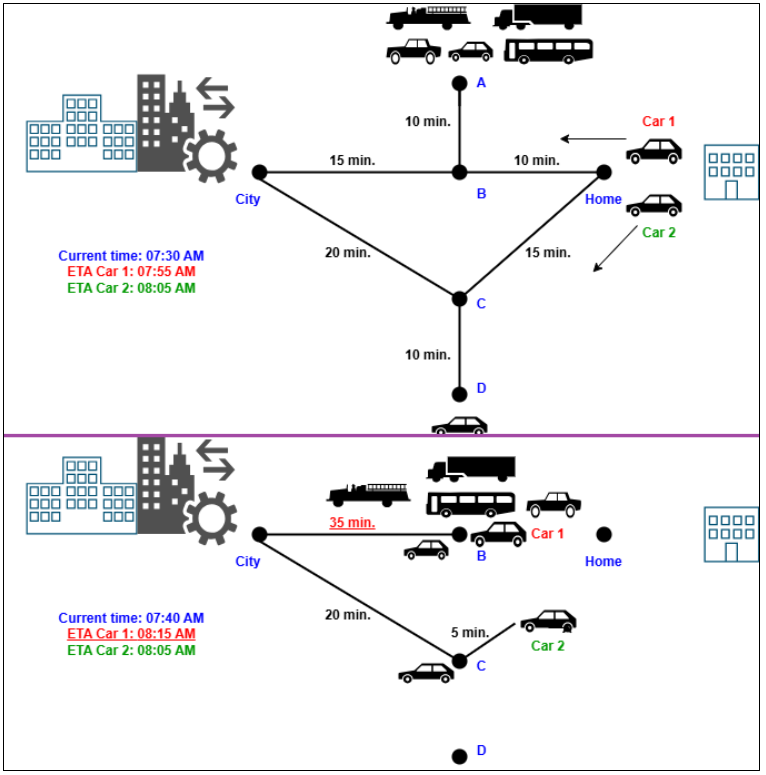
\includegraphics[width=0.63\textwidth]{eta.png}
\caption{Illustration of the ETA prediction challenge: traffic conditions evolve dynamically, causing ETA predictions to change as congestion builds up. Figure adapted from~\cite{SmartSimulativeRoute2025}.}
\label{fig:eta_challenge}
\end{figure}

\subsection{Previous Work in Route-Aware Traffic Prediction}

This research builds upon previous work in traffic prediction and route-aware modeling. Voloch and Voloch-Bloch~\cite{voloch2021} demonstrated real-time future traffic estimations for navigation route optimization, establishing the foundation for dynamic traffic prediction. Voloch et al.~\cite{SmartSimulativeRoute2025} introduced smart simulative route predictions that anticipate future congestion through heuristic simulation, improving ETA accuracy. These works laid the methodological groundwork for graph-based analysis of traffic dynamics and route-aware modeling.

\subsection{State-of-the-Art ETA Prediction Methods}

Machine learning models have been applied to ETA prediction with varying approaches. Tree-based methods such as XGBoost~\cite{chen2016xgboost} leverage handcrafted features and perform well on aggregated trip records, but cannot capture fine-grained spatio-temporal interactions. Trajectory-based neural models address this gap: DeepTTE~\cite{deepTTE2018} learns ETA from raw GPS traces, while STAD~\cite{abbar2020stad} adjusts routing-engine outputs with spatio-temporal corrections. Production systems such as STANN~\cite{stann2021} evaluate on large ride-hailing ETA datasets.

Graph-based spatio-temporal learning has advanced traffic prediction by representing road networks as graphs. DCRNN~\cite{dcrnn2018} combined diffusion graph convolutions with recurrent units, becoming a common backbone for traffic speed/flow prediction on sensor benchmarks (METR-LA~\cite{li2018_metrla}, PEMS-BAY~\cite{pemsbay}). ST-GCN~\cite{yu2018stgcn} introduced spatio-temporal graph convolutional networks, while Graph WaveNet~\cite{wu2019graphwavenet} advanced deep spatial-temporal graph modeling. Most recently, DuETA~\cite{dueta2023} introduced duration-aware ETA modeling at Baidu Maps, categorizing trips into short (0--3 km), medium (3--10 km), and long ($>$10 km) segments, achieving MAEs of 27s, 46s, and 98s respectively. However, DuETA focuses on aggregated road segments rather than individual vehicle trajectories with explicit route intent.

\subsection{Limitations of Existing Approaches}

Existing benchmarks (NYC~\cite{nyc_tlc}, Porto~\cite{moreira2013porto}, Chengdu/DiDi~\cite{didi2016}, Geolife~\cite{zheng2012geolife}) lack explicit representation of pre-planned routes, requiring models to infer paths between origin and destination, introducing ambiguity. Most ETA prediction methods either use static sensor networks (DCRNN~\cite{dcrnn2018}, ST-GCN~\cite{yu2018stgcn}) that aggregate traffic at fixed locations, or rely on trajectory-based learning (DeepTTE~\cite{deepTTE2018}, STAD~\cite{abbar2020stad}) that infers routes implicitly.

Existing datasets present significant constraints: public datasets (NYC Taxi~\cite{nyc_tlc}, Porto Taxi~\cite{moreira2013porto}) lack explicit route information and graph structures, while proprietary datasets (e.g., Baidu Maps used by DuETA~\cite{dueta2023}) are not publicly accessible. The absence of a unified dataset creates a fundamental challenge: trajectory-based models (DeepTTE~\cite{deepTTE2018}, STAD~\cite{abbar2020stad}) require GPS trajectory sequences, static graph models (DCRNN~\cite{dcrnn2018}, ST-GCN~\cite{yu2018stgcn}) require aggregated sensor network data, and route-aware models (DuETA~\cite{dueta2023}) require route segment information. No existing public dataset provides the combination of explicit routes, dynamic graph structure, and vehicle-level data required for evaluating route-aware dynamic graph models, necessitating enhancement of real-world datasets with missing structural features while preserving ground truth travel times.

These limitations highlight the need for approaches that: (1) model traffic at the vehicle level rather than aggregated sensor networks, (2) explicitly encode predefined routes rather than inferring them implicitly, (3) combine dynamic graph structures with temporal learning to capture evolving traffic conditions, and (4) enable evaluation on real-world data by enhancing existing datasets with necessary structural features while maintaining statistical validity and ground truth.


